\chapter{Résultats préliminaires dans un graphe circulaire à $n$ sommets}
\label{Résultats préliminaires}

\section{Inégalité ``triangulaire'' sur les coûts des arêtes}
\label{sec: Inégalité triangulaire}

On se donne un graphe $G=(V,E)$ circulaire à $n$ sommets et un coût $\bs{c} \in \RR^E_+$. On peut alors faire l'hypothèse suivante :
\begin{gather}\label{Inégalité Triangulaire}
  c_{e'}<\sum_{e \in E \backslash \{e'\}} c_e \quad \text{pour tout } e' \in E
\end{gather}

En effet, supposons qu'il existe $e' \in E$ tel que $c_{e'} \ge \sum_{e \in E \backslash \{e'\}} c_e$ $(*)$.

On se donne une solution optimale $(z_e)_{e \in E}$. On note $P = \sum_{e \in E} c_ez_e$ le coût d'une telle solution. On construit alors la séquence de mouvement $(z'_e)_{e \in E}$ par le procédé suivant : chaque passage par l'arête $e'$ est remplacé par un passage sur les autres arêtes avec le même nombre de vélos. Autrement dit, ``on fait le tour dans l'autre sens''. On note $P'$ le coût d'une telle séquence. On a alors :
\begin{align*}
  P' &= \sum_{e \in E \backslash \{e'\}} c_e (z_e + z_{e'}) = \sum_{e \in E \backslash \{e'\}} c_ez_e + \left(\sum_{e \in E \backslash \{e'\}} c_{e}\right)z_{e'} \\
     &\le \sum_{e \in E \backslash \{e'\}} c_ez_e + c_{e'}z_{e'} = P
\end{align*}

Si l'inégalité $(*)$ est stricte, alors nécessairement $z_e = 0$ (sinon, on contredit l'optimalité de la solution), et dans ce cas, nous sommes ramené au cas de la ligne qui est polynomial.

Si l'inégalité $(*)$ est une égalité, alors les deux séquences sont équivalentes et dans ce cas, nous pouvons traiter le problème comme le cas de la ligne.

\section{Borne inférieure de la solution optimale (valable pour un graphe quelconque)}
\label{Borne inf générale}

Nous nous contentons ici de récrire la borne inférieure trouvée par les auteurs de l'article \cite{Benchimol2011}.
\\

Une borne inféieure du SSBP est la solution optimale du programme linéaire en nombre entier dont les variables ``comptent'' le nombre de fois où le camion passe par chaque arête. Les contraintes sont les suivantes :
\begin{enumerate}[label=(\roman*)]
\item les variables sont des entiers naturels.
\item la condition d'Euleur : sauf peut-être en $p$ et en $q$, le camion entre et sort un nombre paire de fois.
\item ``subtour elimination'' : si le camion est en $p \in U \subseteq V $ et qu'il existe des stations non-équilibrée dans $\overline{U}$, alors le camion doit nécessairement traverser $\delta(U)$ au moins une fois (voire plus suivant la position de $q$). Nous utiliserons la notation suivante pour écrire cette contrainte :
\[
\mu(p,q,U,\bs{x},\bs{y}) = \left\{
\begin{array}{ll}
  0 &\mbox{ si } p,q \in U            \mbox{ et } \overline{U} \subseteq B(\bs{x},\bs{y})\\
  0 &\mbox{ si } p,q \in \overline{U} \mbox{ et } U \subseteq B(\bs{x},\bs{y})\\
  1 &\mbox{ si } p \in U              \mbox{ et } q \in \overline{U}\\
  1 &\mbox{ si } p \in \overline{U}   \mbox{ et } q \in U\\
  2 &\mbox{ si } p,q \in U            \mbox{ et } \overline{U} \backslash B(\bs{x},\bs{y}) \ne \emptyset\\
  2 &\mbox{ si } p,q \in \overline{U} \mbox{ et } U \backslash B(\bs{x},\bs{y}) \ne \emptyset
\end{array}
\right.
\]
\item Contrainte de capacité : si $U \subseteq V$ a trop de vélos, le camion doit quitter suffisament de fois $U$ afin de sortir tous ces vélo. Une notation utile est la suivante :
\[
\eta(p,q,U) = \left\{
\begin{array}{ll}
  -1 &\mbox{ si } p \in U            \mbox{ et } q \in \overline{U}\\
  0  &\mbox{ si } p \in U            \mbox{ et } q \in U\\
  0  &\mbox{ si } p \in \overline{U} \mbox{ et } q \in \overline{U}\\
  +1 &\mbox{ si } p \in \overline{U} \mbox{ et } q \in U\\
\end{array}
\right.
\]
\end{enumerate}

Cette borne inférieure est donc solution du programme linéaire en nombre entier
\begin{gather}\label{PLNE borne inf}
\begin{array}{llll}
  \mbox{Min}_{\bs{z}} &\sum_{e \in E} c_ez_e & & \\
  \mbox{s.c.}       &z_e \in \ZZ_+ &\mbox{pour tout } e \in E &\mbox{(i)} \\
                    &z(\delta(v)) \mbox{ est paire} &\mbox{pour tout } v \in V \backslash \{p,q\}&\mbox{(ii)} \\
                    &z(\delta(U)) \ge \mu(p,q,U,\bs{x},\bs{y}) &\mbox{pour tout } U \subseteq V, U \ne \emptyset &\mbox{(iii)} \\
                    &z(\delta(U)) \ge 2 \left\lceil \frac{x(U)-y(U)}{C} \right\rceil\ + \eta(p,q,U) &\mbox{pour tout } U \subseteq V, U \ne \emptyset &\mbox{(iv)}
\end{array}
\end{gather}

\section{Un exemple où la borne inférieure n'est pas atteinte}

\begin{figure}[ht]
  \label{Exemple de borne inf non atteinte}
  \center 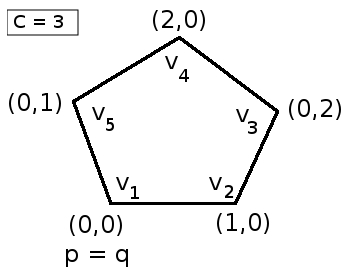
\includegraphics[scale=0.5]{BorneInfNonAtteinte-5sommets.jpg}
  \caption{Exemple de graphe circulaire à 5 sommets où la borne inférieure n'est pas atteinte}
\end{figure}

La solution du programme linéaire en nombre entier \ref{PLNE borne inf} est $\forall e \in E, z_e = 1$. C'est-à-dire qu'il suffirait de faire un tour complet du graphe sans revenir sur ses pas pour l'équilibrer. Or on constate qu'un tel parcours ne peut pas équilibrer le graphe.

Dans le cas général du graphe circulaire à $n$ sommets, on en déduit qu'on ne pourra pas utiliser l'égalité avec la borne inférieure trouvée en section \ref{Borne inf générale} pour démontrer qu'une solution est optimale.

\section{Changement de variables}
\label{Changement variables}

La description de la borne inférieure dans la section \ref{Borne inf générale} donne un minorant de $z(\delta(U))$ pour toute coupe $\delta(U)$ dans le graphe. Dans le cas de l'arbre décrit dans l'article \cite{Benchimol2011}, on avait donc un minorant de $z_e$ pour tout $e \in E$. Comme $c_e$ est positif pour tout $e\in E$, il suffisait de montrer que le minimum de $z_e$ était atteint pour tout $e \in E$ pour montrer que le coût $\sum_{e _in E}c_ez_e$ était minimal.

\begin{prop}\label{Parité coupe}
Soit $G=(V,E)$ un graphe dont tous les sommets sont de degrès paire. Alors toute coupe de G est de cardinal paire.
\end{prop}

Dans le cas d'un graphe circulaire, tous les sommets sont de degrès deux. Par conséquent, selon la proposition \ref{Parité coupe}\footnote{Trouver un lien vers la démonstration ou la mettre en annexe.}, les bornes inférieures des variables $(z_e)_{e \in E}$ ne sont connues que pour des ensembles paires d'arêtes. En supposant connue la valeur de $z(\delta(U))$ pour tout $U \subseteq V$, peut-on retrouver la valeur de $z_e$ pour tout $e \in E$ ?

\begin{lem}\label{Changement de base}
Soit $G=(V,E)$ un graphe circulaire à $n$ sommets. ($n \ge 3$)
On considère le système linéaire suivant d'inconnues $(z_e)_{e \in E}$ :
\begin{gather}\label{Système linéaire complet}
  \sum_{e \in \delta(U)}z_e = z(\delta(U)) \quad \mbox{pour tout } U \subseteq V \mbox{ tel que } U \ne \emptyset
\end{gather}
On suppose que le système \ref{Système linéaire complet} possède au moins une solution.

Alors cette solution est unique.
\end{lem}

La preuve de ce lemme est constructive. On numérote arbitrairement les arêtes du graphe. Il suffit d'extraire le sous-système suivant :
\begin{gather}\label{Système linéaire extrait}
  \left(
  \begin{array}{cccccc}
    1 & 0   & 1 & 0      & \cdots & 0 \\
    1 & 1   &   &        &        &   \\
      & 1   & 1 &        & (0)    &   \\
      &     & 1 & 1      &        &   \\
      & (0) &   & \ddots & \ddots &   \\
      &     &   &        & 1      & 1
  \end{array} \right)
  \left(
  \begin{array}{c}
    z_1 \\
    z_2 \\
    z_3 \\
    z_4 \\
    \vdots \\
    z_n
  \end{array} \right)
  =
  \left(
  \begin{array}{c}
    \zeta_1 \\
    \zeta_2 \\
    \zeta_3 \\
    \zeta_4 \\
    \vdots  \\
    \zeta_n
  \end{array} \right)
\end{gather}

On note $M_n$ la matrice du sytème \ref{Système linéaire extrait}. En développant par rapport à la première ligne, on obtient :
\begin{gather*}
  \mbox{det }M_n =
  1 \times \mbox{det } \left(
  \begin{array}{ccccc}
    1 &                                         &        &        &   \\
    1 & \ddots                                  &        & (0)    &   \\
      & \ddots                                  & \ddots &        &   \\
    \multicolumn{2}{c}{\multirow{2}{*}{ (0) }}  & \ddots & \ddots &   \\
    \multicolumn{2}{c}{}                        &        & 1      & 1
  \end{array} \right)
  + 1 \times \mbox{det } \left(
  \begin{array}{cc|cccc}
    1 & 0                                       & \multicolumn{4}{c}{\multirow{2}{*}{ (0) }} \\
    1 & 1                                       & \multicolumn{4}{c}{}                       \\
    \hline
    \multicolumn{2}{c|}{\multirow{5}{*}{ (0) }} & 1   &        & \multicolumn{2}{c}{\multirow{2}{*}{ (0) }} \\
    \multicolumn{2}{c|}{}                       & 1   & \ddots & \multicolumn{2}{c}{}                       \\
    \multicolumn{2}{c|}{}                       &     & \ddots & \ddots &                                   \\
    \multicolumn{2}{c|}{}                       & (0) &        & 1      & 1
  \end{array} \right)
  = 2
\end{gather*}
Donc le système \ref{Système linéaire extrait} possède une unique solution.
\\

On peut donner une forme explicite de la solution :
\begin{equation}
  \left\{
  \begin{aligned}\notag
    z_1 &= \frac{1}{2}\left(\zeta_1 + \zeta_2 - \zeta_3\right) \\
    z_p &= (-1)^{p-1} z_1 + \sum_{i=2}^p (-1)^{p-i}\zeta_i \quad , \quad \mbox{pour tout } p \in \{2,..,n\}
  \end{aligned}
  \right.
\end{equation}

On obtient ainsi une nouvelle base $\bs{\zeta} = (\zeta_i)_{i \in \{1,..,n\}}$. Nous verrons tout l'intérêt d'un tel changement de variable dans le cas du triangle (section \ref{Cas du Triangle}) et dans le cas où les arêtes ont des coûts unitaires (section \ref{}).
